\begin{table*}[!htb]
\begin{center}\footnotesize
    \resizebox{\textwidth}{!}{%
  \begin{tabular}{@{}l||l|r||r||r|r||r|r|r|r|r||r|r|r|r@{}}
  \hline
  \multicolumn{1}{c||}{} & \multicolumn{3}{c||}{Data characteristics} & \multicolumn{3}{c||}{\# Patterns} & \multicolumn{4}{c||}{Micro-F} & \multicolumn{4}{c}{Macro-F} \\ \hline \hline
  \multicolumn{1}{c||}{Dataset} &\multicolumn{1}{c|}{\#Features} & \multicolumn{1}{c|}{\#FI} & \multicolumn{1}{c||}{$n$} & DDP & MPP & EPM & Orig & DDP & MPP & EPM & Orig & DDP & MPP &EPM \\ \hline
  \hline
  %\small car & $21$ & $1728$ & $3$ & $95$ & $65$ & $96.2$ & $96.1$ & $99.9$ & $99.4$ & $49.0$ &$49.0$ & $99.8$ & $96.1$ \\
  \small cmc & $(0/2/7)$ & $24$ & $1473$ & $4$ & $99$ & $23$ & $77.5$ & $77.4$ & $76.2$ & $77.3$ & $57.3$ & $57.1$ & $57.7$ & $59.4$ \\
  %\small ticTacToe & $27$ & $958$ &  $11$ & $270$ & $92$ & $98.3$ & $98.3$ & $100$ & $100$ & $98.1$ & $98.1$ & $100$ & $100$ \\
  %\small flare & $(0/0/11)$ & $27$ & $1066$ & $2$ & $430$ & $86$ & $92.3$ & $93.3$ & $92.7$ & $92.6$ & $49.6$ & $48.3$ & $66.3$ & $61.6$\\ 
  \small nursery  & $(0/0/8)$ & $27$ & $12690$ & $4$ & $258$ & $198$ & $97.5$ & $98.2$ & $99.9$ & $99.8$ & $49.4$ & $79.4$ & $99.8$ & $98.8$\\
  %\small crx   & $28$ & $653$& $3$ & $145$ & $55$ & $83.7$ & $85.7$ & $86.3$ & $86.2$ & $83.9$ & $85.9$ & $86.4$ & $86.3$\\
  \small sick & $(6/1/22)$ & $36$ & $2800$ & $5$ & $627$ & $89$ & $94.6$ & $94.7$ & $96.1$ & $95.8$ & $62.6$ & $64.8$ & $81.0$ & $75.6$\\
  \small kr-v-k & $(0/0/16)$ & $40$ & $28056$ & $7$ & $71$ & $63$ & $99.1$ & $99.1$ & $99.6$ & $99.6$ & $49.8$ & $49.8$ & $87.8$ & $88.4$ \\
  %\small hypo & $3$ & $433$ & $113$ & $96.3$ & $97.8$ & $98.6$ & $98.4$ & $71.9$ & $86.6$ & $91.7$ & $90.4$\\
  \small german & $(0/7/13)$ & $51$ & $1000$ & $8$ & $548$ & $97$ & $70.7$ & $70.9$ & $73.1$ & $72.7$ & $49.6$ & $55.2$ & $65.3$ & $64.2$\\ 
  %\small fars & $67$ & $100968$& - & - & $2071$ & $99.2$ & - & - & $99.5$ & $70.5$ & - & - & $85.3$\\
  \small connect-4 & $(0/0/42)$ & $75$ & $67557$ & - & - & $907$ & $90.5$ & - & - & $90.5$ & $47.5$ & - & - & $56.6$\\ 
  \small census & $(1/12/28)$ & $76$ & $299284$ & - & - & $5618$& $93.8$ & - & - & $93.8$ & $48.4$ & - & - & $51.6$ \\
  \small poker & $(0/10/0)$ & $85$ & $1025010$ & - & - & $14216$ & $23.1$ & - & - & $49.6$ & $22.4$ & - & - & $44.5$ \\ 
  \end{tabular}
 }
   \caption[Evaluating the informativeness of DDPMine, MPP and EPM patterns]{Evaluating the informativeness of DDPMine, MPP and EPM patterns on standard datasets.}
  \label{tab:performance}
 \end{center}
\end{table*}
\section{Why Use EPM?}
In this section, we explain why EPM is a better alternative compared to its counterparts for large NLP datasets.
%show that EPM is a practical algorithm for large datasets.
We compare EPM with two efficient discriminative pattern mining algorithms, i.e.\
Minimal Predictive Patterns (MPP) \cite{batal10} and Direct Discriminative Pattern Mining (DDPMine) \cite{cheng08},
on standard machine learning datasets.
%\footnote{Given that MPP and DDPMine were not applicable to our coreference data.}. 

MPP selects patterns that are significantly more predictive than all their sub-patterns.
It measures significance by the binomial distribution.
For each pattern of length $l$, MPP checks $2^l-1$ sub-patterns.
DDPMine is an iterative approach that selects 
the most discriminative pattern at each iteration and reduces 
the search space of the next iteration by removing all samples that include 
the selected pattern. DDPMine uses the FP-Tree structure.

We show that EPM scales best and compares favorably based on the informativeness of resulting patterns.
Due to its efficiency, EPM can handle large datasets similar 
to ones that are commonly used in various NLP tasks.
%
\subsection{Experimental Setup}
%For evaluation, we implement 
%DDPMine \cite{cheng08} and MPP \cite{batal10}.
%We use approximated MPP in our experiments.
%It is a variant of MPP 
%that achieves higher efficiency by 
%using a lossy pruning technique \cite{batal10}.
We use the same FP-Tree implementation for DDPMine and EPM.
In all algorithms, we consider a pattern as frequent if it occurs in 10\% of the samples of one of the classes.
%We use 
%Equation~\ref{eq:freq} as the frequency condition and $\lambda_1=0.1$ for all three approaches unless otherwise stated.
We use $\Theta_l=3$ for both MPP and EPM.

We perform 5-times repeated 5-fold cross validation and the results are averaged.
In each validation, all experiments are performed on the same split.
We use a linear SVM, i.e.\  LIBLINEAR 2.11 \cite{fan08}, as the baseline classifier.
%\footnote{\url{https://www.csie.ntu.edu.tw/~cjlin/liblinear/}} 
%and the performance is evaluated using micro- and macro-averaged F$_1$.

We use several datasets from the UCI machine learning repository \cite{Lichman:2013} whose
characteristics are presented in the first three columns of Table~\ref{tab:performance},
i.e.\ the number of (1) (real/integer/nominal) features (\#Features), (2) frequent items (\#FI), and (3) samples ($n$). 
We use one[the minority class]-vs-all technique for datasets with more than two classes.
%We do not use binning methods for converting real or integer features to nominal ones. 
\subsection{How Informative are EPM Patterns?}
To evaluate the informativeness of mined patterns,
the common practice is to add them as new features to the feature set of the baseline classifier;
the more informative the patterns, the greater impact they would have on the overall performance.
All patterns are added as binary features, i.e.\ 
the feature is true for samples that contain all items of the corresponding pattern.

The effect of the patterns of DDPMine, MPP and EPM on the overall accuracy 
is presented in Table~\ref{tab:performance}.  
The columns \#Patterns show the number of patterns mined by each of the algorithms. 
The \emph{Orig} columns
show the results of the SVM using the original feature sets.
The \emph{DDP}, \emph{MPP}, and \emph{EPM} columns show the results of the SVM 
on the datasets for which the feature set is extended by 
the features mined by DDPMine, MPP, and EPM, respectively.
The results of the 5-repeated 5-fold cross validation are reported
if each single validation takes less than 10 hours. 

Based on the results of Table~\ref{tab:performance} (1) EPM efficiently scales to larger datasets,
(2) MPP and EPM patterns considerably improves the performance,
and (3) EPM has on-par results with MPP while it mines considerably fewer patterns.
\subsection{How Does it Scale?}
\begin{figure}[!htb]
\begin{center}
%\resizebox {\columnwidth} {!} {
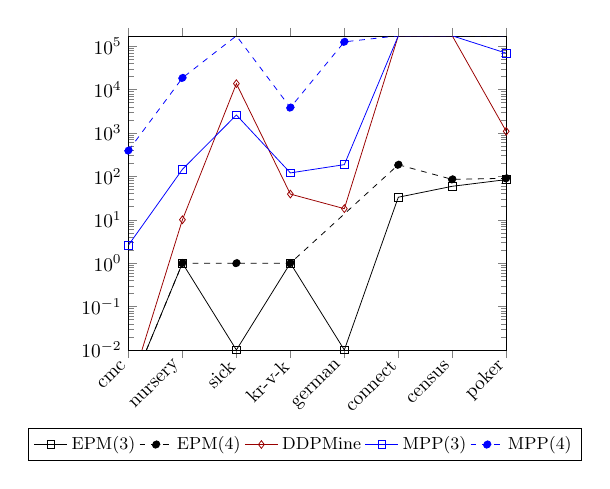
\begin{tikzpicture}[scale = .7]   %
\begin{axis}[
ymin = 0.01, ymax= 170000, legend entries = {EPM(3)\\EPM(4)\\ DDPMine\\ MPP(3)\\MPP(4)\\},ymode=log, %ylabel = Mining Time (Seconds),
legend columns=5, 
legend style={at={(1.2,-0.25)},font=\small}, legend cell align=center,
 draw=none,
 xtick=data,
 xticklabel = {\benchmark{\tick}},
 xtick align=outside,
 ytick align=inside,
 x tick label style={rotate=45,anchor=east},
 title style={font=\Large},
 ylabel near ticks,
 enlarge x limits=false,
xtick distance={400},
 symbolic x coords={cmc,nursery,sick,kr-v-k,german,connect,census,poker},
 ymajorgrids=true,
 grid = none,
 ]
\addplot[
    solid,
    color=black,
    mark=square,
    ]
    coordinates {
    (cmc, 0.001)(nursery, 1)(sick, 0.01)(kr-v-k, 1)(german, 0.01)(connect, 33)(census, 59)(poker, 84)
    };
    \addplot[
    dashed,
    color=black,
    mark=*,
    ]
    coordinates {
    (cmc, 0.001)(nursery, 1)(sick, 1)(kr-v-k, 1)(german,0)(connect, 185)(census, 85)(poker, 90)};
   %     \addplot[
   % dashed,
   % color=black,
   % mark=triangle,
   % ]
   % coordinates {
   % (cmc, 0.001)(nursery, 1)(sick, 3)(kr-v-k, 2)(german,3)(connect, 108)(census, 269)(poker, 238)};
    \addplot[
    solid,
    color=red!60!black,
    mark=diamond,
    ]
    coordinates {
    (cmc, 0.001)(nursery, 10)(sick, 13663)(kr-v-k, 39)(german, 18)(connect, 172800)(census, 172800)(poker, 1090) };
    \addplot[
    color=blue,
    mark=square,
    ]
    coordinates {
    (cmc, 2.6)(nursery, 145)(sick, 2589)(kr-v-k, 120)(german, 186)(connect, 172800)(census, 172800)(poker,68794) };
    \addplot[
    dashed,
    color=blue,
    mark=*,
    ]
    coordinates {
    (cmc, 394)(nursery, 18515)(sick, 172800)(kr-v-k, 3833)(german,125514)(connect, 172800)(census, 172800)(poker, 172800) };

 \end{axis}
\end{tikzpicture}
\end{center}
%}
\caption{Comparison of mining times (seconds).}
\label{fig:all}
\end{figure}
Figure~\ref{fig:all} compares EPM mining time (in seconds) with those of DDPMine and MPP.
The parameter in the parentheses is the pattern size threshold, e.g.\ $\Theta_l=4$ for EPM(4).
The experiments that take more than two days are terminated and are not included.
%TODO As can be seen, increasing $\Theta_l$ does not notably affect the running time of EPM 
%on the datasets with smaller search spaces.
%TODO However, on the datasets with a larger number of frequent items, 
%decreasing $\lambda_1$ affects the processing time more than increasing $\Theta_l$. 
EPM is notably faster in comparison to the other two approaches.
It is notable that the examined datasets are considerably smaller than the coreference data, which includes more than 33 million samples and 200 frequent feature-values.